\documentclass{article}

\usepackage{listings}
\usepackage{xcolor}
\usepackage{courier}
\usepackage{graphicx}
\usepackage{float}

\definecolor{lightgray}{gray}{0.95}

\lstset{
	basicstyle=\ttfamily,
	backgroundcolor=\color{lightgray},
	numbers=left,
	tabsize=3,
	frame=tblr,
	keywordstyle=\color{blue},
	morekeywords={graph, digraph, shape, node}
}

\title{Graphviz for State Diagrams}
\date{2021-04-10}
\author{Raha Moradi Shahmiri\\raham9619@gmail.com}



\begin{document}
	\pagenumbering{gobble}
	\maketitle
	\newpage

	\pagenumbering{arabic}

	\section{Introduction}
	Graphviz is a popular opensource tool for visualizing graphs, as its name suggests. In this tutorial, we use it for drawing state diagrams. Thus, we shall be equiped with a powerful tool for designing and illustrating state machines. Graphviz is a package with many capabilities, from which we only use dot, which parses dot language and produces graph visualizations. 
	\newline
	From the DOT description, many output formats may be generated. One way to generate PNG images, suitable for many usecases, is the following command:
	\newline \newline
	
	\textbf{\lstinline{dot -Tpng [input file name] -o [output file name]}}

	\section{Basic Notation}
	Graphviz uses DOT Language to describe graphs. A simple DOT description is shown in listing \ref{lst:dot1}.

	\lstinputlisting[caption={Sample graph description},label={lst:dot1} ]{listing1.dot}
	
	\begin{figure}[H]
		\begin{center}
			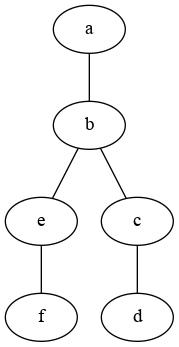
\includegraphics[width=25mm]{figure1.png}
		\end{center}
		\caption{dot output for listing \ref{lst:dot1}.}
		\label{fig:png1}
	\end{figure}

	Lets investigate the above code.
	
	\subparagraph{Graph declaration}
		Graph must be declared. Its name comes in "double quotes." The keyword \lstinline{digraph} can also be used, indicating a digraph, eg. a directed graph.
	
	\subparagraph{Edge declaration}
		Undirected edges are declared using \lstinline{--} operator. For directed edges, \lstinline{<-} is used. Mixing directed and undirected edges is not supported: Directed edges should only be used in digraphs, while undirected edges should only be used in graphs.

	\subparagraph{Node declaration}
		Nodes can be implicitly or explicitly declared. In this snippet, they are declared implicitly, through edge definitions.
	
	\subsection{Edge Attributes}
	In general, attributes for nodes, edges and graphs can be assigned using braces, \lstinline{[ ]}. Some common attributes for edges are demonstrated in listing \ref{lst:dot2}.

	\lstinputlisting[caption={Demonstration of some edge attributes},label={lst:dot2} ]{listing2.dot}

	\begin{figure}[H]
		\begin{center}
			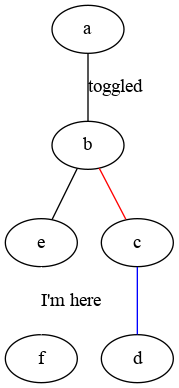
\includegraphics[width=25mm]{figure2.png}
		\end{center}
		\caption{dot output for listing \ref{lst:dot2}.}
		\label{fig:png2}
	\end{figure}

	Here, \lstinline{color} and \lstinline{label} attributes of edges have been illustrated. 

	\subsection{Node Attributes}
	Nodes can also have attributes. In this specific application, we usually would like to choose their shapes, for aesthetic reasons as well as highlighting special nodes. In addition to defining node-specific attributes, it's possible to define global attributes for nodes, which hold true, unless overriden by their node-specific counterparts. The same holds true for edges.

	\lstinputlisting[caption={Demonstrating of node shapes},label={lst:dot3} ]{listing3.dot}

	\begin{figure}[H]
		\begin{center}
			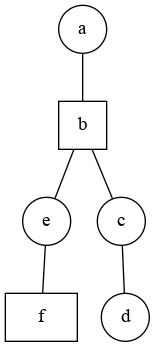
\includegraphics[width=25mm]{figure3.png}
		\end{center}
		\caption{dot output for listing \ref{lst:dot3} }
		\label{fig:png3}
	\end{figure}

	It can be seen that \lstinline{node} defines global attributes.

	\subsection{Common Colors}

	\subsection{Common Node Shapes}

\end{document}
